%%%%%%%%%%%%%%%%%%%%%%%%%%%%%%Packages%%%%%%%%%%%%%%%%%%%%%%%%%%%%%%
\documentclass[12pt,a4paper]{article}							   %
\usepackage[left=2cm, right=2cm, top=2cm, bottom=2cm]{geometry}	   %
%\usepackage{booktaps}											   %
\usepackage[usenames, dvipsnames]{color}						   %
\usepackage{color}												   %
\newcommand{\dbar}{d\hspace*{-0.08em}\bar{}\hspace*{0.1em}}		   %
\usepackage{amsthm,amssymb,amsmath}	  							   %
\usepackage{hyperref}
\hypersetup{
    colorlinks=true,
    linkcolor=cyan,
    filecolor=magenta,      
    urlcolor=blue,
}											   %
\usepackage{graphicx,wrapfig}			   					       %
\usepackage{xepersian}			   								   %
\settextfont{B Nazanin}											   %
\defpersianfont\titr[Scale=1]{XB Zar}	  						   %
%%%%%%%%%%%%%%%%%%%%%%%%%%%%%%Packages%%%%%%%%%%%%%%%%%%%%%%%%%%%%%%

%%%%Text%%%%
\begin{document}
%%%%section*{مبانی ریاضیاتی  نظریه ترمودینامیک}%%%%
\begin{center}

\section*{مبانی ریاضیاتی ترمودینامیک
\lr{$Mathematical~Foundations~of~Thermodynamics$}}

\end{center}

\thispagestyle{plain}
ریاضیات ابزار و زبان فیزیکدانان در جهت توصیف طبیعت بوده؛ لذا لازم است هر فیزیک پیشه‌ای با این زبان آشنا باشد. 

در این فصل به مقدمات ریاضیاتی ترمودینامیک پرداخته شده و لازمه کار برای مطالعه این نظریه قدرتمند فیزیک به طور مختصر بررسی شده است.
\\
%%%%subsection{چند قضیه در مشتقات جزئی}%%%%
\subsection{دو قضیه در مشتقات جزئی
\lr{$(Two~Theorems~in~Partial~Derivatives)$}}
فرض کنید سه مغیر
$x, y, z$
  توسط رابطه زیر بهم مربوط هستند:
\begin{align*}
F(x,y,z)=0
\end{align*}
به طور مثال:
$x^{2}+y^{2}+z^{2}-2=0$
که معادله یک دایره به شعاع
$\sqrt{2}$
در فضای ۳ بعدی دکارتی است.
\\
علی الاصول می‌شود یکی از دو متغیر را بر حسب دیگری نوشت (هرچند که ممکن است این کار از نظر عملی دشوار باشد):
\begin{align*}
x=x(y,z)
\end{align*}
دیفرانسیل کامل
$x$
به صورت زیر خواهد بود:
\begin{equation}\label{Re1}
dx=\left(\dfrac{\partial{x}}{\partial{y}}\right)_{z}dy+\left( \dfrac{\partial{x}}{\partial{z}}\right)_{y}dz
\end{equation}
که در آن:
\begin{equation*}
\left( \dfrac{\partial{x}}{\partial{y}}\right)_{z}=\lim_{h\to\ 0} \dfrac{x(y+h,z)-x(y,z)}{h}
\end{equation*}
بدین معنا که
$y$
اجازه تغییر کوچکی به اندازه
$h$
داشته باشد در حالی که
$z$
ثابت بماند.
مجددا می‌توان همین کار را برای
$z$
کرد طوری که این بار
$z=z(x,y)$
پس خواهیم داشت:
\begin{align}\label{Re2}
dz=\left( \dfrac{\partial{z}}{\partial{x}}\right)_{y}dx+\left( \dfrac{\partial{z}}{\partial{y}}\right)_{x}dy
\end{align}
حال در رابطه
\eqref{Re1}
به جای
$dz$
رابطه
\eqref{Re2}
را قرار می‌دهیم و خواهیم داشت:
\begin{align}\label{Re3}
\boxed{\textcolor{blue}{dx=\left(\dfrac{\partial x}{\partial z}\right)_{y}\left(\dfrac{\partial z}{\partial x}\right)_{y}dx+\left[ \left(\dfrac{\partial x}{\partial y}\right)_{z}+\left(\dfrac{\partial x}{\partial z}\right)_{y}\left(\dfrac{\partial z}{\partial y}\right)_{x}\right]dy}}
\end{align}
هر جفت ۲تایی از
$x, y, z$
را که به عنوان متغیرهای مستقل برگزینیم در معادله بالا صدق می‌کنند.


حال در رابطه
\eqref{Re3}
فرض کنید مقدار
$ dy=0 , dx\neq 0 $
بدین ترتیب خواهیم داشت:
\begin{align*}
dx=\left(\dfrac{\partial x}{\partial z}\right)_{y}\left(\dfrac{\partial z}{\partial x}\right)_{y}dx
\end{align*}
با حذف
$ dx$
از طرفین رابطه خواهیم داشت:
\begin{align}\label{Re4}
\boxed{\textcolor{blue}{\left(\dfrac{\partial x}{\partial z}\right)_{y}=\dfrac{1}{\left(\dfrac{\partial z}{\partial x}\right)_{y}}}}
\end{align}
\par
این تساوی که به
\textbf{قضیه وارون}
 معروف است، اصلا بدیهی نبوده و در حالت کلی برای مشتقات جزئی نمی‌توان چنین معکوس پذیری را انجام داد و به عبارتی باید ثابت مشتق گیری برای هر دو مشتق یکسان باشد (که در اینجا
$ y $
است)، تا چنین رابطه‌ای صحت ریاضیاتی یابد. اما رابطه زیر همواره برقرار است:
\begin{align}
\boxed{\textcolor{blue}{\dfrac{dx}{dz}=\dfrac{1}{\dfrac{dz}{dx}}}}
\end{align}
و این تفاوت اساسی میان
$ d $
با
$\partial  $
است.

بیان مثالی از مشتق گیری جزئی در بین روابطی که در تبدیل بین دو دستگاه مختصات دکارتی و استوانه‌ای است می‌تواند 
تفاوت را به وضوح روشن کند.\\
\par
در فضای سه بعدی می‌توان مختصات هر نقطه را در دستگاه‌های مختصات مختلفی بیان کرد. دو دستگاه پرکاربرد برای حل مسائل بسته به تقارن‌های موجود در مسئله؛ دکارتی و استوانه‌ای هستند. در دستگاه دکارتی برای نمایش هر نقطه از سه طول استفاده می‌شود و در دستگاه استوانه‌ای از دو طول و یک زاویه. به این ترتیب که در شکل زیر می‌بینید.\\
\begin{figure}[h!]
\centering
\includegraphics*[height=5cm]{Im1}
\caption
{
دستگاه مختصات استوانه‌ای با پارامترهای
$\rho,\varphi,z$
}
\end{figure}
\\
از هندسه شکل مشخص است که روابط زیر بین پارامترهای توصیف کننده دو دستگاه حاکم است:
\begin{align*}
x=\rho \cos \varphi,~~~~y=\rho \sin \varphi,~~~~z=z
\end{align*}
و روابط معکوس به شرح زیر خواهد بود:
\begin{align*}
\rho=\sqrt{x^{2}+y^{2}},~~~~y=tan^{-1} \left( \dfrac{y}{x}\right) ,~~~~z=z
\end{align*}
به سه مشتق جزئی زیر دقت کنید:
\begin{align*}
\left(\dfrac{\partial x}{\partial \rho}\right)_{\varphi}=\cos \varphi\\
\left(\dfrac{\partial \rho}{\partial x}\right)_{y}=\cos \varphi\\
\left(\dfrac{\partial \rho}{\partial x}\right)_{\varphi}=\dfrac{1}{\cos \varphi}
\end{align*}
تفاوت به وضوح پدید آمد که مشتق جزئی با ثابت‌‌های متفاوت چگونه پاسخ‌های متمایزی دارد.
\\
برای یافتن قضیه دوم اینبار در رابطه
\eqref{Re3}
فرض کنید
$ dx=0 , dy\neq 0 $
خواهیم داشت بدین ترتیب خواهیم داشت:
\begin{align}\label{Re5}
\left(\dfrac{\partial x}{\partial y}\right)_{z}+\left(\dfrac{\partial x}{\partial z}\right)_{y}\left(\dfrac{\partial z}{\partial y}\right)_{x}=0
~\Rightarrow~
\left(\dfrac{\partial x}{\partial y}\right)_{z}=-\left(\dfrac{\partial x}{\partial z}\right)_{y}\left(\dfrac{\partial z}{\partial y}\right)_{x}
\end{align}
با استفاده از قصیه وارون که در رابطه
\eqref{Re4}
به آن دست یافتیم می‌توان رابطه
\eqref{Re5}
را به صورت زیر نوشت:
\begin{align}
\left(\dfrac{\partial x}{\partial y}\right)_{z}=-\dfrac{1}{\left(\dfrac{\partial z}{\partial x}\right)_{y}}\dfrac{1}{\left(\dfrac{\partial y}{\partial z}\right)_{x}}
~\Rightarrow~
\boxed{\textcolor{blue}{\left(\dfrac{\partial x}{\partial y}\right)_{z}\left(\dfrac{\partial y}{\partial z}\right)_{x}\left(\dfrac{\partial z}{\partial x}\right)_{y}=-1}}
\end{align}
به رابطه موجود در کادر
\textbf{قضیه وارونگی}
گویند.\\
یکی دیگر از نتایج رابطه
\eqref{Re5}
اتحاد زیر خواهد بود که بسیار جالب و مهم است به خصوص در ترمودینامیک:
\begin{align}\label{Re6}
\boxed{\textcolor{blue}{\left(\dfrac{\partial x}{\partial y}\right)_{z}=-\dfrac{\left(\dfrac{\partial x}{\partial z}\right)_{y}}{\left(\dfrac{\partial y}{\partial z}\right)_{x}}}}
\end{align}
\\
به رابطه
\eqref{Re6}
دقت کنید، در سمت چپ رابطه مقدار
$ z $
ثابت است و اجازه تغییر ندارد در حالی که در سمت راست در صورت و مخرج این مقدار اجازه تغییر دارد. این اتحاد در یافتن متغیرهای ترمودینامیکی در فصل هفتم بسیار کاربردی خواهد بود.
\subsection{ترتیب مشتق گیری
\lr{$(Order~of~Derivatives)$}}
\begin{wrapfigure}{r}{5cm}
\label{wrap-fig:1}
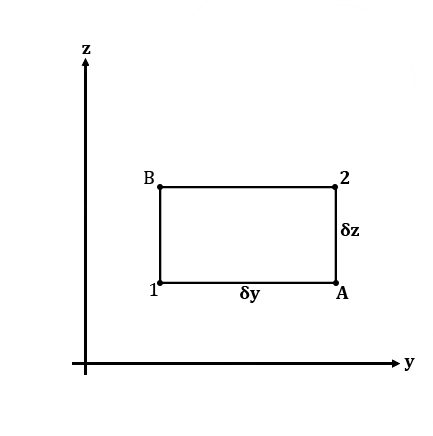
\includegraphics[width=5.5cm]{Im2}
\end{wrapfigure}
مجددا فرض کنید
$ x=x(y,z) $
. برای تغییرات کوچک
$ y, z $
می‌توانیم
$ x $
را به صورت یک سری تیلور بر حسب پارامترهایش بسط داد.
از دو مسیر به نقطه ۲ می‌رویم دقت کنید ابتدا از نقطه ۱ از طریق
$ A $
به نقطه ۲ و سپس از طریق
$ B $
به نقطه ۲ می‌رویم. مجداد دقت کنید اینها مسیرهایی هستند که
$ y $
یا
$ z $
ثابتند و مقدار
$ x $
تابع دو متغیر
$ y,z$
است.
\begin{align}\label{Re7}
\begin{split}
curve:1\rightarrow A\rightarrow 2 : ~ ~ x_{A}=\sum_{n=0}^{\infty}\dfrac{1}{n!}\left( \dfrac{\partial^{n}x}{\partial y^{n}}\right)_{z}(\delta y)^{n}\\
\vert_{x=x_{1}} ~~= x_{1}+\left( \dfrac{\partial x_{1}}{\partial y}\right)_{z}(\delta y)+\dfrac{1}{2!}\left( \dfrac{\partial^{2}x_{1}}{\partial y^{2}}\right)_{z}(\delta y)^{2}+\cdot \cdot \cdot
\end{split}
\end{align}
\par
\begin{equation}\label{Re8}
x_{2}=\sum_{n=0}^{\infty}\dfrac{1}{n!}\left( \dfrac{\partial^{n}x}{\partial z^{n}}\right)_{y}(\delta z)^{n}
~~\vert_{x=x_{A}} ~~=x_{A}+\left( \dfrac{\partial x_{A}}{\partial z}\right)_{y}(\delta z)+\dfrac{1}{2!}\left( \dfrac{\partial^{2}x_{A}}{\partial z^{2}}\right)_{y}(\delta z)^{2}+\cdot \cdot \cdot 
\end{equation}
حال با جایگذاری
$ x_{A} $
از معادله
\eqref{Re7}
در معادله
\eqref{Re8}
خواهیم داشت:
\begin{align}\label{Re9}
\begin{split}
x_{2}=x_{1}&+\left( \dfrac{\partial x_{1}}{\partial y}\right)_{z}(\delta y)+\left( \dfrac{\partial x_{1}}{\partial z}\right)_{y}(\delta z)+\dfrac{1}{2!}\left( \dfrac{\partial^{2}x_{1}}{\partial y^{2}}\right)_{z}(\delta y)^{2}\\
	       &+\dfrac{1}{2!}\left(\dfrac{\partial^{2}x_{1}}{\partial z^{2}}\right)_{y}(\delta z)^{2}+					\dfrac{\partial}{\partial z}\left( \dfrac{\partial x_{1}}{\partial y}\right)_{z}(\delta y)(\delta z)+\mathcal{O}(\delta ^{n})~~~~,n\geq 3
\end{split}
\end{align}
که منظور از
$ \mathcal{O}(\delta ^{n}) $
جملاتی از مرتبه ۳ به بالاست که بخاطر کوچک بودن
$ \delta $
آنها را نادیده می‌گیریم.
\\
حال از طریق
$ B $
به نقطه ۲ می‌رویم با محاسبات مشابهی خواهیم داشت:
\begin{align}\label{Re10}
\begin{split}
curve:1\rightarrow B\rightarrow 2 : x_{2}=x_{1}&+\left( \dfrac{\partial x_{1}}{\partial y}\right)_{z}(\delta y)+\left( \dfrac{\partial x_{1}}{\partial z}\right)_{y}(\delta z)+\dfrac{1}{2!}\left( \dfrac{\partial^{2}x_{1}}{\partial y^{2}}\right)_{z}(\delta y)^{2}\\											    										   &+\dfrac{1}{2!}\left(\dfrac{\partial^{2}x_{1}}{\partial z^{2}}\right)_{y}(\delta z)^{2}+					\dfrac{\partial}{\partial y}\left( \dfrac{\partial x_{1}}{\partial z}\right)_{y}(\delta z)(\delta y)+\mathcal{O}(\delta ^{n})~~~~,n\geq 3
\end{split}
\end{align}
واضح است که معادلات
\eqref{Re9}
و
\eqref{Re10}
باید باهم یکسان باشند پس برای این باید جمله آخر هر دو معادله برابر باشند. لذا خواهیم داشت:
\begin{align*}
\boxed{\textcolor{blue}{\dfrac{\partial}{\partial y}\left( \dfrac{\partial x}{\partial z}\right)_{y}=\dfrac{\partial}{\partial z}\left( \dfrac{\partial x}{\partial y}\right)_{z}}}
\end{align*}
و یا
\begin{align}\label{Re11}
\boxed{\textcolor{blue}{ \dfrac{\partial ^{2} x}{\partial z \partial y}= \dfrac{\partial ^{2} x}{\partial y \partial z}}}
\end{align}
و این نشان می‌دهد برای این موجود فرقی ندارد که ابتدا نسبت به کدام متغیرش مشتق می‌گیرید و اصطلاحا نسبت به مرتبه مشتق گیری ناورداست. به چنین
$ x $
ای
دیفرانسیل کامل گویند.
\\
\subsection{دیفرانسیل کامل و تابع حالت
\lr{$(Exact~Differential~\&~State~Function)$}}
به موجودی که تغییراتش به صورت زیر بیان شود دیفرانسیل کامل گویند:
\begin{align}
dx=\left(\dfrac{\partial{x}}{\partial{y}}\right)_{z}dy+\left( \dfrac{\partial{x}}{\partial{z}}\right)_{y}dz
\end{align}
شرط لازم و کافی دیفرانسیل کامل بودن همان معادله
\eqref{Re11}
است.
\\
به بیانی موجودی که دیفرانسیل کامل باشد تابع مسیر نیست و به عبارتی موجوداتی که دیفرانسیل کامل باشند‫‪،‬‬ تغییراتشان تابع حالت ابتدایی و نهایی خواهد بود و به جزئیات مسیری که پیموده شده ربطی نخواهند داشت.
\\
\subsection{دیفرانسیل ناکامل و تابع مسیر
\lr{$(Inexact~Differential~\&~Process~Function)$}}
دیفرانسیل‌های ناکامل تابع مسیر می‌باشند و تغییراتشان به جزپیات مسیر پیموده شده ربط دارد.
\par
از منظر ریاضیاتی هیچ تابع
$ u $
وجود ندارد که
$ u=\int du $
باشد. به بیان ریاضیاتی دقیق‌تری؛ برای یک میدان برداری
$ \overrightarrow{U} $
که یک دیفرانسیل ناکامل باشد هیچ تابع
$ \Phi$
نمی‌توان یافت که:
$ \overrightarrow{U}=\overrightarrow{\nabla}\Phi  $
باشد.
\\
\par
از منظر این نگاه دقیق ریاضیاتی، مثال فیزیک جالبی وجود دارد؛ می‌دانیم که برای نیروهای پایستار، پتانسیل‌هایی وجود دارد که گرادیان آنها نیرو را به ما می‌دهد. به طور مثال برای نیروی کولن و یا گرانشی به ترتیب پتانسیل‌های کولنی و گرانشی وجود دارد. اما برای نیرویی نظیر اصطکاک چه؟! آیا تا بحال دیده‌اید که پتانسیلی برای این نیرو بیان شود؟ پتانسیل اصطکاکی وجود ندارد تا گرادیان آن نیروی اصطکاک شود پس نیروی اصطکاک یک دیفرانسیل ناکامل است.
\\
مثال جالب دیگر فیزیکی جابه‌جایی و مسیر پیموده شده در مکانیک است؛ در سینماتیک وقتی می‌خواستیم جابه‌جایی را بیابیم فقط دو نقطه انتها و ابتدا را از هم کم می‌کردیم، اما برای مسیر پیموده شده این کار اشتباه است مثلا اگر مسیری را برویم و به نقطه آغاز برگردیم واضح است که جابجایی صفر است اما آیا مسیر پیموده شده صفر است؟ خیر مسیر  پیموده شده نیز یک دیفرانسیل ناکامل است.
\\
در ترمودینامیک نقش دیفرانسیل‌های ناکامل بسیار پر رنگ است. تغییرات انرژی درونی سیستم به صورت تغییرات کار و گرما است:
\begin{align*}
dU=\dbar W+\dbar Q
\end{align*}
که در آن انرژی درونی
$ (U) $
دیفرانسیل کامل بوده و در طی یک فرآیند‫‪،‬‬ تغییرات آن فقط به حالت ابتدا و انتهای فرآیند وابسته است و مستقل از مسیر است اما
کار
$ W $
و گرما
$ Q $
دیفرانسیل ناکامل بوده و تابع مسیری است که سیستم در طی فرآیند پیموده است. تغییرات این دو را با
$\dbar$
نمایش می‌دهیم که تفاوت این دو را با
$U$
قائل شویم.
\\
\par
به طور مثال انفجار یک ترقه را متصور شوید که توسط کار و گرما صورت گرفته و با تغییرات انرژی در یک محیط همراه بوده است. تغییر انرژی محیط به شما نحوه انتقال انرژی را نمی‌دهد و به شما این اطلاع را نخواهد داد که به طور مثال ترقه با چه میزان گرما و به چه ضربه مکانیکی منفجر شده است و تغییر انرژی فقط به حالت آن محیط قبل و بعد از انفجار مربوط است. در حالی که کار و گرما بستگی دارند به اینکه به چه طریقی انفجار صورت گرفته است و تابع مسیرند.
\newpage
\subsection*{منابع}
\begin{flushleft}
\lr{Equilibrium Thermodynamics (Book by C. Adkins)}\\
\lr{Heat and Thermodynamics (Book by Mark Zemansky)}\\
\lr{\href{https://en.wikipedia.org/wiki/Inexact_differential}{Inexact Differential - Wikipedia}}\\
\lr{\href{http://mathworld.wolfram.com/InexactDifferential.html}{Inexact Differential - Mathworld.Wolfram}}\\
\lr{\href{https://en.wikipedia.org/wiki/Exact_differential}{Exact Differential - Wikipedia}}\\
\lr{\href{http://mathworld.wolfram.com/ExactDifferential.html}{Exact Differential - Mathworld.Wolfram}}\\
\lr{\href{https://en.wikipedia.org/wiki/State_function}{State Function - Wikipedia}}\\
\lr{\href{https://en.wikipedia.org/wiki/Process_function}{Process Function - Wikipedia}}\\
\end{flushleft}

\begin{flushleft}
\lr{Thermodynamics and Statistcal Mechanics 1 - Fall 2018 -- Teacher: Dr. Afshin Montakhab}
\lr{Provided ‌‌‌by TA of the class, Ehsan Kiani. Email: \href{EhKiani96@gmail.com}{\underline{EhKiani96@gmail.com}}}
\end{flushleft}

\end{document}

